% DRAFT (2026-11-28) for the coordinator's read. Not published.
\documentclass[11pt]{amsart}
\usepackage[margin=1.05in]{geometry}
\usepackage{amssymb,amsmath,graphicx,booktabs,xcolor}
\usepackage{hyperref}
\emergencystretch=2em
\hypersetup{colorlinks=true,linkcolor=blue!50!black,citecolor=blue!50!black,urlcolor=blue!50!black}
\newtheorem{theorem}{Theorem}
\newtheorem{lemma}{Lemma}
\theoremstyle{remark}\newtheorem*{remark}{Remark}
\newcommand{\R}{\mathbb{R}}

\title[Chaotic geodesics in the Manko--Novikov spacetime]{Chaotic geodesics in the Manko--Novikov spacetime:\\ a computer-assisted proof and a Melnikov theorem (AI-assisted)}
\author{Sumit Pal}
\address{Independent researcher}
\urladdr{https://orcid.org/0009-0000-9541-2793}
\date{28 November 2026. Draft.}

\begin{document}
\begin{abstract}
We prove that timelike geodesics of the Manko--Novikov spacetime---the Kerr black hole deformed by an anomalous mass
quadrupole $\beta$---are chaotic on an energy level near an unstable spherical orbit: for mass $M=5$, spin $a=3$ and
$\beta=3/100$ the stable and unstable manifolds of a hyperbolic periodic orbit intersect transversally, so the return
map has a Smale horseshoe and the geodesic flow on that level has positive topological entropy. The proof is
computer-assisted, using interval arithmetic throughout. We also prove, by a Melnikov-type argument resting on an
interval-certified Fourier coefficient, that the same conclusion holds for every $0<|\beta|<\beta_0$ of either sign,
with $\beta_0>0$ not computed. The decision arithmetic of the first proof was re-evaluated in a second arithmetic
library, the field was re-derived from the published metric by a separate implementation, and the same code applied
to Kerr ($\beta=0$) correctly finds no transversality. No value of the entropy is claimed. This work was AI-assisted;
the independent checks were carried out by separate AI sessions and systems, not by human peer review.
\end{abstract}

\maketitle

\section{Introduction}
The Kerr metric is the unique stationary, asymptotically flat vacuum black hole of general relativity, and its
geodesic flow is completely integrable: besides the energy $E$, the axial angular momentum $L$ and the mass shell, it
conserves the Carter constant~\cite{Carter}. ``Bumpy'' spacetimes that deviate from Kerr through a higher multipole
are used to test this uniqueness with gravitational waves from extreme-mass-ratio inspirals; for them a fourth
integral is generally absent, and chaotic orbits would leave observable imprints such as resonance plateaus in the
frequency evolution~\cite{GLM,ALC}.

The Manko--Novikov (MN) spacetime~\cite{MN} is an exact stationary axisymmetric vacuum solution that reduces to Kerr
when its anomalous quadrupole parameter $\beta$ vanishes~\cite{GLM}. Numerical studies found chaotic and ergodic
orbits in MN on surfaces of section and by rotation numbers~\cite{GLM,ALC,CLA}; the non-integrability argument in
this literature is the absence of a Carter-like constant, not a proof. Rigorous chaos results exist for other
perturbed black-hole geodesic problems by Melnikov-type arguments~\cite{Moeckel,BC,LV,PS}. Computer-assisted proofs of
homoclinic chaos are established in celestial mechanics, e.g.~\cite{CKMJ}. To our knowledge, the results below are the
first computer-assisted proof of chaos for Manko--Novikov geodesics (the searches are listed in the software
record~\cite{Software}, \texttt{NOVELTY\_CHECK.md}).

\section{Setting}
We use the MN metric in the form of Gair, Li and Mandel~\cite[eqs.~(2)--(5)]{GLM}, in prolate spheroidal coordinates
$(t,x,y,\phi)$ with $\rho=k\sqrt{(x^2-1)(1-y^2)}$, $z=kxy$, parameters $k=4$, $\alpha=-1/3$ (so $M=5$, $a=3$) and
$\beta$. Timelike geodesics with $p_t=-E$, $p_\phi=L$ reduce to the two-degree-of-freedom Hamiltonian
$H(x,y,p_x,p_y)=\tfrac12\big(g^{xx}p_x^2+g^{yy}p_y^2\big)+V_{E,L}(x,y)$ on the shell $H=-\tfrac12$. Throughout,
\[ E=0.93528150456799871854,\qquad L=12.972532035607280691, \]
the level of an unstable inclined spherical Kerr orbit at $r=M+kx=16$ (the level is certified in~\cite{MelRes}).
The section is $\Sigma=\{y=0,\ \dot y>0\}$ with coordinates $(x,p_x)$; $P_\beta:\Sigma\to\Sigma$ is the first-return
map, real-analytic and area-preserving. The map $R:(x,y,p_x,p_y)\mapsto(x,-y,-p_x,p_y)$ is a time-reversing symmetry
of the flow for every $\beta$, and acts on $\Sigma$ as $(x,p_x)\mapsto(x,-p_x)$; its fixed set on $\Sigma$ is
$\{p_x=0\}$.

\section{Results}
\begin{theorem}[$\beta=3/100$]\label{thm:1}
For $\beta=3/100$, $P_\beta$ has a hyperbolic fixed point $w$ (the periodic orbit near $r\approx16$) with
\[ |w-(2.784144616590083788,\,0)|_\infty\le10^{-19}, \]
and a point $p=(x_p,0)\in W^u(w)\cap\{p_x=0\}$ with
\[ x_p\in[10.58222772208632,\ 10.58222772208635] \]
at which $W^u(w)$ and $W^s(w)$ intersect transversally. Consequently
an iterate of $P_\beta$ has a horseshoe (a hyperbolic invariant Cantor set conjugate to the full 2-shift), and the
geodesic flow on this level has positive topological entropy.
\end{theorem}

\begin{theorem}[all small $\beta$]\label{thm:2}
For the same $M,a,E,L$ there is $\beta_0>0$ such that for every $\beta$ with $0<|\beta|<\beta_0$ the continuation of the
$R$-symmetric homoclinic orbit at Melnikov phase $\psi_*=3\pi/2$ is transversal; hence the conclusions of
Theorem~\ref{thm:1} hold for every such $\beta$. The bound $\beta_0$ is not computed; Theorem~\ref{thm:2} does not
reach $\beta=3/100$, which Theorem~\ref{thm:1} covers separately.
\end{theorem}

Both theorems use the following elementary criterion.
\begin{lemma}[reversible transversality]\label{lem:A1}
Let $p\in W^u(w)\cap\mathrm{Fix}(R)$ and let $v=(v_x,v_{p_x})$ span $T_pW^u$. Since $R$ maps $W^u$ onto $W^s$,
$T_pW^s$ is spanned by $Rv=(v_x,-v_{p_x})$; hence $W^u\pitchfork W^s$ at $p$ if and only if $v_x\neq0$ and $v_{p_x}\neq0$.
\end{lemma}

\section{Proof of Theorem~\ref{thm:1}: method}
\emph{Fixed point.} A Newton--Krawczyk argument~\cite[Thm.~30]{CKMJ} for $P(w)-w$ on a ball of radius $10^{-19}$ gives
$Y=1.55\cdot10^{-21}$, $Z=2.89\cdot10^{-8}$, $Zr-r+Y<0$. The enclosed derivative has trace $26.7986\ldots$ and
determinant $1$, so the eigenvalues are $\lambda_u\approx26.76$ and $\lambda_u^{-1}$.

\emph{Local unstable manifold.} In a frame of approximate eigenvectors, cone conditions on a box of half-width
$\delta=10^{-9}$ give an expansion rate $\mu\ge26.75$ and contraction $\nu\le0.821$; a cone lemma (stated and proved in
the record) then encloses $W^u_{\rm loc}$ as a graph of slope $\le L_c=1.203\cdot10^{-2}$ over $|u|\le\delta^*=3.735\cdot10^{-11}$.
The lemma used is the following; its proof (cone invariance, backward contraction off the cone, and a
continuation argument) is in the record (\texttt{PREREG.md}, amendment A11).

\begin{lemma}[cone lemma]\label{lem:cone}
In affine coordinates $(u,s)$ let $P$ be $C^1$ near $B=\{|u|\le\delta,\ |s|\le\delta\}$, with a fixed point
$p^*=(u^*,s^*)$, $|u^*|,|s^*|\le\rho'$, and let $\left[\begin{smallmatrix}a&b\\c&d\end{smallmatrix}\right]$ be an interval
matrix containing $DP(\xi)$ for every $\xi\in B$. If for some $L>0$
\[ \mu:=a_{\min}-|b|_{\max}L>1,\qquad |c|_{\max}+|d|_{\max}L\le L\mu,\qquad \nu:=|c|_{\max}/L+|d|_{\max}<1, \]
then $W^u(p^*)$ contains the graph $\{(u,h(u)):|u-u^*|\le\delta^*\}$ of a $C^1$ function with $|h'|\le L$ and
$h(u^*)=s^*$, where $\delta^*=(\delta-\rho')/(\kappa\max(1,L))$ and $\kappa=a_{\max}+|b|_{\max}L$.
\end{lemma}

\begin{table}[h]
\centering\footnotesize\setlength\tabcolsep{4pt}
\begin{tabular}{@{}lccc@{}}
\toprule
 & MN, $\beta=3/100$ & Kerr, $\beta=0$ & sabotaged MN\\
 & (Theorem~\ref{thm:1}) & (control i) & (control iii)\\
\midrule
fixed point $Y$ & $1.55\cdot10^{-21}$ & $1.16\cdot10^{-21}$ & $1.56\cdot10^{-21}$\\
fixed point $Z$ & $2.9\cdot10^{-8}$ & $1.1\cdot10^{-8}$ & $2.4\cdot10^{-8}$\\
cone slope $L$ & $1.203\cdot10^{-2}$ & $1.036\cdot10^{-2}$ & $1.202\cdot10^{-2}$\\
reach $\delta^*$ & $3.735\cdot10^{-11}$ & $3.721\cdot10^{-11}$ & $3.735\cdot10^{-11}$\\
half BVP $Y$ & $7.8\cdot10^{-16}$ & $6.6\cdot10^{-16}$ & $7.8\cdot10^{-16}$\\
half BVP $Z$ & $3.4\cdot10^{-4}$ & $3.0\cdot10^{-4}$ & $3.4\cdot10^{-4}$\\
half BVP $r$ & $1.2\cdot10^{-14}$ & $1.0\cdot10^{-14}$ & $1.2\cdot10^{-14}$\\
$v_x$ & $[1.1245,1.1300]\cdot10^{7}$ & $[-2.24,2.24]\cdot10^{4}$ & $[1.1243,1.1298]\cdot10^{7}$\\
$0\in v_x$? & no: transversal & yes, as required & no\\
\bottomrule
\end{tabular}
\caption{The three certificates computed by the same code (printed values; full enclosures in the record).}
\label{tab:cert}
\end{table}

\emph{Symmetric half boundary-value problem.} We solve for $(u,z_1,\dots,z_8)\in\R^{17}$ such that the point of
$W^u_{\rm loc}$ with unstable coordinate $u$ is mapped by $P$ through the nodes $z_1,\dots,z_8$ to a point on
$\{p_x=0\}$ ($m=9$ maps; the last includes a long excursion to the outer turning point). A Newton--Krawczyk argument
uniform over the manifold's enclosure gives $Y=7.84\cdot10^{-16}$, $Z=3.42\cdot10^{-4}$, radius $r=1.20\cdot10^{-14}$:
a unique solution, hence the point $p$ of Theorem~\ref{thm:1}.

\emph{Transversality.} Pushing the unstable tangent (with its cone uncertainty) through the certified derivatives of the
nine maps gives
\[ v_x\in[1.12449\cdot10^{7},\ 1.13004\cdot10^{7}],\qquad v_{p_x}\in[-3.58821\cdot10^{11},\ -3.58821\cdot10^{11}], \]
both excluding $0$; Lemma~\ref{lem:A1} gives transversality. The ratio $v_x/|v|\approx3.13\cdot10^{-5}$ agrees with a
floating-point prediction ($3.1258\cdot10^{-5}$). The Smale--Birkhoff homoclinic theorem~\cite{Smale} gives the
horseshoe; positivity of the entropy passes to the flow because return times are bounded on the compact invariant set.

\emph{Arithmetic.} All enclosures use CAPD~\cite{CAPD} with MPFR 128-bit intervals, Taylor order 20 and a
Lohner-type set representation. A compile-time guard rejects any non-MPFR interval type; every enclosure that enters a
decision is checked finite before use (interval multiplication can otherwise absorb a NaN---we found and fixed this
during the work and repeated all runs, with identical results). Every integration step certifies that the orbit stays
in the region where the metric is regular and Lorentzian ($x-1\ge0.05$, $\det g<0$, $g_{\phi\phi}>0$), and each return
certifies the crossing direction and $H=-\tfrac12$.

\section{Proof of Theorem~\ref{thm:2}: the Melnikov route}
At $\beta=0$ the separatrix $\Gamma_0=W^u=W^s$ lies in a level set of the radial Kerr integral
$K_r=\tfrac12\big[\Delta p_r^2-\mathcal P(r)^2/\Delta+r^2\big]$, with $r=M+kx$, $p_r=p_x/k$, $\Delta=r^2-2Mr+a^2$ and
$\mathcal P=E(r^2+a^2)-aL$; along geodesics in Mino time $\lambda$ ($d\tau=\Sigma\,d\lambda$) the polar motion has
frequency $\Upsilon_\theta$ and phase $\psi$. The first-order
displacement of $W^u_\beta$ and $W^s_\beta$, measured by $K_r$ on a transversal at Mino $\theta$-phase $\psi_0$, is
$\beta M(\psi_0)+O(\beta^2)$ with $M=\Upsilon_\theta L'$ (Robinson~\cite[Thm.~3.4, Rem.~3.10]{Robinson}; we checked its
hypotheses against this setting at source). Here
\[ L(\psi_0)=L_0+2\sum_{m\ge1}L_{2m}\cos(2m\psi_0),\qquad \Upsilon_\theta=15.0122754941\ldots, \]
and the coefficients were enclosed in interval arithmetic (Arb~\cite{Arb}) along the Kerr homoclinic loop~\cite{MelRes}:
\[ L_2=-4.77482114974644\cdot10^{-5}\pm6.8\cdot10^{-20},\qquad |L_2|-4|L_4|-T_3>1.524\cdot10^{-5}, \]
where $T_3\ge\sum_{m\ge3}m^2|L_{2m}|$ is a certified Cauchy-estimate tail bound. Hence
$|L''(3\pi/2)|\ge8(|L_2|-4|L_4|-T_3)>1.2\cdot10^{-4}$, and $M$ vanishes only at $\psi_0\in\frac\pi2\mathbb Z$, all
nondegenerate (Figure~\ref{fig:split}). Let $t(\beta)=v_x/v_{p_x}$ be the slope of $W^u_\beta\cap\Sigma$ at the
$R$-symmetric point $p(\beta)$, which continues analytically by the implicit function theorem. Comparing $W^u_\beta$
with its $R$-image $W^s_\beta$ on $\Sigma$ gives the exact first-order relation
\[ t'(0)=\frac{\Upsilon_\theta^{2}\,L''(\psi_*)}{2k^2F_t^2},\qquad F_t=\partial_r\!\left[\tfrac12\big(r^2-\mathcal P(r)^2/\Delta(r)\big)\right]_{r=r_t}, \]
with $r_t$ the outer turning radius; numerically $t'(0)\approx-1.003\cdot10^{-3}$. Since $t(0)=0$ and $t'(0)\neq0$,
$t(\beta)\neq0$ for small $\beta\neq0$, and Lemma~\ref{lem:A1} gives transversality. As checks: floating-point slopes
$t/\beta=1.0119\cdot10^{-3}$ ($\beta=10^{-2}$) and $1.0419\cdot10^{-3}$ ($3\cdot10^{-2}$) extrapolate to within
$0.6\%$ of $t'(0)$, the rigorous slope at $\beta=3/100$ from Theorem~\ref{thm:1} is $t\in[-3.1494,-3.1338]\cdot10^{-5}$,
and a separate AI system derived the same constant independently from the discrete-map form of the Melnikov
method~\cite{DRR}.

\begin{figure}[t]
\centering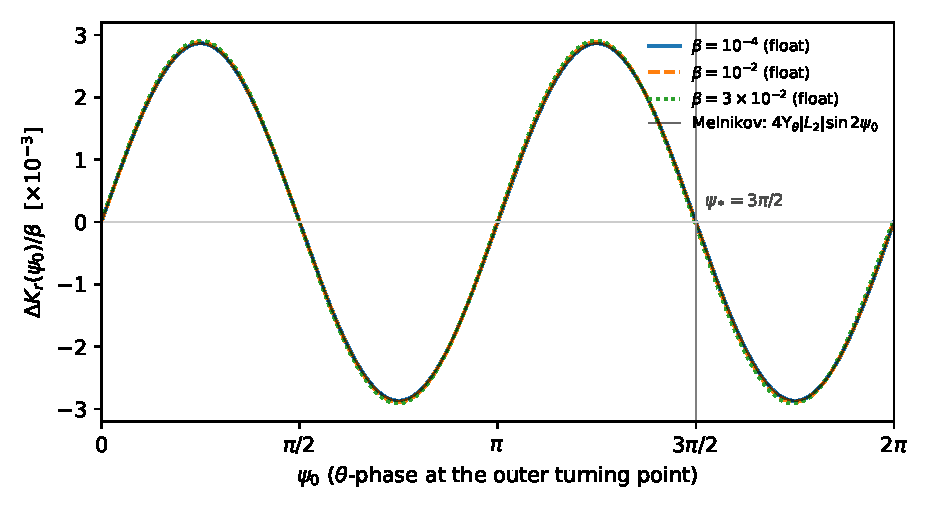
\includegraphics[width=0.82\textwidth]{fig_splitting.pdf}
\caption{Illustrative (floating point, not part of the proof). The splitting $\Delta K_r(\psi_0)/\beta$ between
$W^u_\beta$ and $W^s_\beta$ for three values of $\beta$, against the first-order Melnikov prediction
$4\Upsilon_\theta|L_2|\sin2\psi_0$ with the certified $L_2$. The zero used in both theorems is $\psi_*=3\pi/2$.}
\label{fig:split}
\end{figure}

\section{Verification}
\begin{itemize}
\item \textbf{Controls.} (i) Kerr ($\beta=0$), same code: $v_x\in[-2.24\cdot10^4,\,2.24\cdot10^4]$ contains $0$, as
integrability requires; MN's $v_x$ lies $\sim500$ times outside Kerr's enclosure (relative to $|v|$). (ii) Kerr's
homoclinic points are certified to form a continuous arc (a parametric Newton--Krawczyk argument plus the exact Carter
bracket). (iii) A field with one $\beta^2$ term removed certifies a symmetric point disjoint from MN's by
$1.3\cdot10^{-6}$. (iv) The validator reproduces Capi\'nski--Kepley--Mireles James's homoclinic proof in the planar
restricted three-body problem~\cite[Thm.~3]{CKMJ}.
\item \textbf{Second arithmetic library.} Every inequality decided in Theorem~\ref{thm:1} and controls (i)--(iii) was
re-evaluated from exact dumps of the enclosures in python-flint/Arb~\cite{Arb} (256-bit), with exact rational coverage
checks. Deliberately corrupted inputs (NaN/$\infty$, a flipped sign, a perturbed point image, a shrunk box) were
rejected. The checker was written from the stated formulas by the same AI session that wrote the main code, and read
by a separate AI session.
\item \textbf{Independent field.} A separate AI agent, without access to our code, implemented the reduced Hamiltonian
from~\cite{GLM} in mpmath. It agrees with the field used in both proofs to $4\cdot10^{-46}$ (relative to scale) at 97
points along the orbit for $\beta\in\{0,\pm3/100\}$, and a field with the $\beta^2$ term removed was rejected. Both
sides resolved a typesetting ambiguity in~\cite[eq.~(3h)]{GLM} the same way, consistent with the vacuum Einstein
equations.
\item \textbf{Decision rules fixed before each computation.} The decision rules, controls and expected outcomes were
written and committed before each run.
\end{itemize}

\section{Limits}
No value or lower bound of the topological entropy is claimed; only one energy level, one spin and one orbit family
are treated; $\beta_0$ in Theorem~\ref{thm:2} is not explicit. The flow and derivative enclosures rest on a single
validated integrator (CAPD); a second integrator has not been run. The Melnikov coefficients rest on a single interval
implementation (Arb). Lemma~3.8 of~\cite{Robinson}, which underlies the cited Theorem~3.4, is proved
in~\cite{RobinsonETDS}, which we did not read. The cone lemmas and the theorem glue were checked by a separate AI
session; no external expert has yet read the proofs.

\section{Reproducibility}
Code, specifications, outputs and checkers are in the software record~\cite{Software}, in the directories
\begin{center}\texttt{qsim/mn\_homoclinic\_spike/}\quad and\quad \texttt{qsim/mn\_melnikov/}.\end{center}
Versions: CAPD (git 2f06098), MPFR 4.2.2,
GMP 6.3.0, python-flint 0.9.0, mpmath 1.3.0, Python 3.13 on macOS (Apple silicon). Rerunning Theorem~\ref{thm:1} takes
about 1.6 core-hours (controls about 4 more); the Arb re-evaluation and the field comparison take seconds; the Melnikov
certificates took about 2.5 and 24 hours. A referee guide in the record lists which file proves which statement.

\section*{AI assistance}
This work was carried out with substantial assistance from AI systems: Claude (Anthropic) and Gemini (Google). They
were used for writing and running code, deriving and checking mathematics, literature searches and drafting text,
under the direction of the author. All checks described here as independent were done by separate AI sessions or
systems; none is human peer review. No external expert has yet read the proofs.

\begin{thebibliography}{99}
\bibitem{Arb} F.~Johansson, Arb: efficient arbitrary-precision midpoint-radius interval arithmetic, IEEE Trans.\ Comput.\ 66 (2017) 1281--1292.
\bibitem{ALC} T.~A.~Apostolatos, G.~Lukes-Gerakopoulos, G.~Contopoulos, How to observe a non-Kerr spacetime using gravitational waves, Phys.\ Rev.\ Lett.\ 103 (2009) 111101, doi:10.1103/PhysRevLett.103.111101.
\bibitem{BC} L.~Bombelli, E.~Calzetta, Chaos around a black hole, Class.\ Quantum Grav.\ 9 (1992) 2573--2599, doi:10.1088/0264-9381/9/12/004.
\bibitem{CAPD} T.~Kapela, M.~Mrozek, D.~Wilczak, P.~Zgliczy\'nski, CAPD::DynSys: a flexible C++ toolbox for rigorous numerical analysis of dynamical systems, arXiv:2010.07097.
\bibitem{Carter} B.~Carter, Global structure of the Kerr family of gravitational fields, Phys.\ Rev.\ 174 (1968) 1559--1571, doi:10.1103/PhysRev.174.1559.
\bibitem{CKMJ} M.~J.~Capi\'nski, S.~Kepley, J.~D.~Mireles James, Computer assisted proofs for transverse collision and near collision orbits in the restricted three body problem, arXiv:2205.03922.
\bibitem{CLA} G.~Contopoulos, G.~Lukes-Gerakopoulos, T.~A.~Apostolatos, Orbits in a non-Kerr dynamical system, Int.\ J.\ Bifurc.\ Chaos 21 (2011) 2261, arXiv:1108.5057.
\bibitem{DRR} A.~Delshams, R.~Ram\'irez-Ros, Poincar\'e--Melnikov--Arnold method for analytic planar maps, Nonlinearity 9 (1996) 1--26, doi:10.1088/0951-7715/9/1/001.
\bibitem{GLM} J.~R.~Gair, C.~Li, I.~Mandel, Observable properties of orbits in exact bumpy spacetimes, Phys.\ Rev.\ D 77 (2008) 024035, doi:10.1103/PhysRevD.77.024035, arXiv:0708.0628.
\bibitem{LV} P.~S.~Letelier, W.~M.~Vieira, Chaos in black holes surrounded by gravitational waves, Class.\ Quantum Grav.\ 14 (1997), doi:10.1088/0264-9381/14/5/026.
\bibitem{MN} V.~S.~Manko, I.~D.~Novikov, Generalizations of the Kerr and Kerr--Newman metrics possessing an arbitrary set of mass-multipole moments, Class.\ Quantum Grav.\ 9 (1992) 2477--2487, doi:10.1088/0264-9381/9/11/013.
\bibitem{MelRes} S.~Pal (AI-assisted), certified Melnikov coefficients for the MN quadrupole, in~\cite{Software}, \texttt{qsim/mn\_melnikov/RESULT.md}.
\bibitem{Moeckel} R.~Moeckel, A nonintegrable model in general relativity, Commun.\ Math.\ Phys.\ 150 (1992) 415--430, doi:10.1007/BF02096667.
\bibitem{PS} J.~Polcar, O.~Semer\'ak, Free motion around black holes with discs or rings: between integrability and chaos.\ VI.\ The Melnikov method, Phys.\ Rev.\ D 100 (2019) 103013, doi:10.1103/PhysRevD.100.103013.
\bibitem{Robinson} C.~Robinson, Melnikov method for autonomous Hamiltonians, Contemp.\ Math.\ 198 (1996) 45--53, doi:10.1090/conm/198/02519.
\bibitem{RobinsonETDS} C.~Robinson, Horseshoes for autonomous Hamiltonian systems using the Melnikov integral, Ergodic Theory Dynam.\ Systems 8 (1988) 395--409, doi:10.1017/S0143385700009500.
\bibitem{Smale} S.~Smale, Diffeomorphisms with many periodic points, in: Differential and Combinatorial Topology, Princeton Univ.\ Press (1965) 63--80, doi:10.1515/9781400874842-006.
\bibitem{Software} S.~Pal, vestigium v2026.11.28 (software, AI-assisted), Zenodo, doi:10.5281/zenodo.24602464.
\end{thebibliography}
\end{document}
